% Created 2025-01-03 Fri 18:51
% Intended LaTeX compiler: pdflatex
\documentclass[11pt]{article}
\input{../../../preamble.tex}
% setting up title page
\title{
  
\includegraphics[width=0.4\textwidth]{fmf_logo}\\
  {\small Oddelek za fiziko} \\
  {Difuzija}\\
  {\small Poročilo pri FP5}\\

}
\date{}
\author{ Kristofer Č. Povšič, 28211104 \\[5 cm]
 \small  Asistent: Tilen Knaflič \\
}

\addbibresource{refs.bib}
\begin{document}

\maketitle
\newpage
\tableofcontents

\section{Uvod}\label{sec:org7496756}
\subsection{Pot žarka v nehomogene, plastovitem sredstvu}\label{sec:org81f2c64}
Lomni zakon se posploši na sredstvo z zvezno spremenljivim lomnim količnikom

\[ \cos \phi = \frac{\text{konst}}{n(x)}
\]

Prehod žarka skozi kiveto izračunamo kot

\begin{equation}
\label{eq:1}
\frac{\mathrm{d} \phi}{\mathrm{d} x} = \frac{1}{n} \frac{\mathrm{d} n}{\mathrm{dz} }
\end{equation}

Žarki se torej odklonijo za kot \(\alpha_N = \frac{d}{n} \frac{\mathrm{d} n}{\mathrm{dz}}\). Po izstopu iz kivete se odklon še poveča za \(\alpha_Z = n \alpha_N\) Na zaslonu dobimo odmik \(Y = bd \frac{\mathrm{d} n}{\mathrm{dz}}\). Če je sredstvo homogeno, dobimo na zaslonu premico.

Koncentracija difundirajoče snovi \(f\) je funkcija kraja in časa. Difuzijski tok je sorazmeren gradientu koncetracije \(\vec{Q} = - D \nabla f\). Ob upoštevanju še konitnuitetne enačbe \(\nabla \vec{Q} = -\frac{\partial f}{\partial t}\) dobimo \emph{difuzijsko enačbo}:

\begin{equation}
\label{eq:2}
D \nabla ^2 f = \frac{\partial f}{\partial t}
\end{equation}

oz. v našem primeru:

\begin{equation}
\label{eq:3}
D \frac{\partial ^2 f}{\partial z ^2} = \frac{\partial f}{\partial t}
\end{equation}

Osnovna rešitev te enačbe je

\begin{equation}
\label{eq:4}
f = \frac{1}{\sqrt{4 \pi Dt}} e^{- \frac{z ^2}{4Dt}}
\end{equation}

To je rešitev za porazdelitev, ko je ob času \(t = 0\) vsa difundirajoča snov zbrana na mestu \(z=0\). Rešitev za poljubno začetno porazdelitev snovi dobimo iz osnovne rešitve z integriranjem. V našem primeru imamo na začetku snov, ki je enakomerno porazdeljena po polprostoru \(z > 0\), kjer je \(f(z) = 1\) in \(f(z) = 0\) za \(z< 0\). Rešitev je neka čudna funkcija. Ob sklepanju, da je lomni količnih linearna funkcija koncentracije dobimo odmik kot

\begin{equation}
\label{eq:5}
Y = bd (n_1 - n_0)
\end{equation}

Ploščina pod krivuljo pa je od časa neodvisna:

\begin{equation}
\label{eq:6}
S = \int\limits_{}^{} y \,\mathrm{d z} = kbd(n_1 - n_0), \quad k = \frac{a + b}{a}
\end{equation}

\subsection{Potrebščine}\label{sec:orgbc5db6b}
\begin{itemize}
\item zaslon
\item optična klop
\item kiveta z alkoholom in vodo
\item steklena palčka
\item laser
\item milimetrski papir
\end{itemize}

\subsection{Naloge}\label{sec:orga510493}
\begin{itemize}
\item preveri časovno neodvisnost ploščine \(S\)
\item določi difuzijsko konstanto \(D\)
\end{itemize}
\section{Meritve in izračuni}\label{sec:org161f0a0}

\subsection{Konstanta ploščine}\label{sec:org31b401e}

S pomočjo Web Plot Digitizerja (vir \cite{noauthor_webplotdigitizer_nodate}) sem označil točke na grafu in dobil vrednost grafov v pikslih. Izmeril sem tudi, koliko pikslov vsebuje en kvadratni centimeter in preko tega dobil površino grafa v kvadratnih centimetrih.

Za 3 različne čase sem dobil konstantne vrednosti znotraj napake

\begin{tabela}
  \centering
\[
  \begin{array}{|c|c|} \hline
    t [\mathrm{min}] & S [\mathrm{cm} ^2] \\ \hline
   0 & (18.6 \pm 0.1) \\
    33.5 & (18.0 \pm 0.4) \\
    70.0 & (19.5 \pm 0.7) \\ \hline
  \end{array}
\]
\caption{\small Izmerjene površine grafov za tri različne čase.}
\end{tabela}

Preko enačbe \ref{eq:6} dobimo pa vrednost

\[ S = (19.2 \pm 0.1) \mathrm{cm} ^2
\]
\subsection{Difuzijska konstanta}\label{sec:orga79e3ef}

Z izmerjenimi vrednosti \(Y_{max}\) sem narisal graf \(\frac{1}{4 \pi k ^2} \left( \frac{S}{Y_{max}} \right)^2\) v odvisnosti od časa.

\begin{slika}[H]
  \centering
  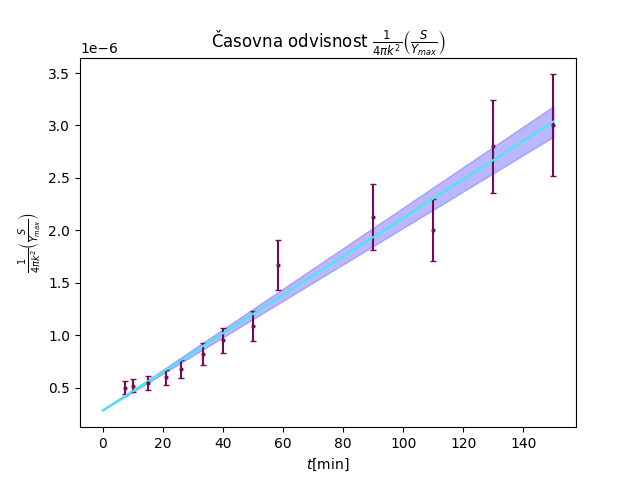
\includegraphics{./figures/DifKonstanta.png}
  \caption{\small Graf prikazuje izmerjene vrednosti maksimalne višine pri difuziji v odvisnosti od časa.}
\end{slika}

Naklon premice je difuzijska konstanta \(D\) in v našem primeru je vrednost naklona regresivne premice enak

\[ k = (1.8 \pm 0.1) 10^{-8} \frac{\mathrm{m} ^2}{s}
\]
\section{Komentar}\label{sec:org58c18e0}

Postavitev vaje je bila precej enostavna, ampak samo zaradi tega, ker sem imel dobre nasvete: difuzijo sem pripravil pri umivalniku, kjer lahko komolce postaviš na tla in imaš tako precej bolj mirne roke.

Iskal sem difuzijsko konstanto na spletu za primerjavo, vendar nisem našel nič vrednega.

\printbibliography[heading=bibintoc]
\end{document}
